\documentclass{article}

\usepackage[final]{neurips_2019}

\usepackage[utf8]{inputenc}
\usepackage[T1]{fontenc}
\usepackage{hyperref}
\usepackage{url}
\usepackage{booktabs}
\usepackage{amsfonts}
\usepackage{nicefrac}
\usepackage{microtype}
\usepackage{graphicx}
\usepackage{xcolor}
\usepackage{lipsum}
\usepackage{subfig}
% \usepackage[nomarkers,nolists,figuresonly]{endfloat} %comment out when finish
\usepackage{amsmath}
\usepackage{booktabs}
\usepackage{multirow}
\usepackage{float}


\newcommand{\note}[1]{\textcolor{blue}{{#1}}}

\title{
  SemiBERT: Enhancing Multitask Learning in NLP through Semi-Supervised Techniques \\
  \vspace{1em}
  \small{\normalfont Stanford CS224N Default Project}  % Select one and delete the other
}

\author{
  Danhua Yan \\
  Department of Computer Science \\
  Stanford University \\
  \texttt{dhyan@stanford.edu} \\
  % Examples of more authors
%   \And
%   Name \\
%   Department of Computer Science \\
%   Stanford University \\
%   \texttt{name@stanford.edu} \\
%   \And
%   Name \\
%   Department of Computer Science \\
%   Stanford University \\
%   \texttt{name@stanford.edu}
}

\begin{document}

\maketitle

\begin{abstract}
  SemiBERT, a method enhancing multitask NLP learning with the Unsupervised Data 
  Augmentation (UDA) framework, is introduced in this paper. Utilizing BERT's inherent 
  \texttt{[SEP]} token for sentence-pair encoding notably improves performance. Moreover, 
  the exponential schedule in TSA effectively regulates overfitting, paving the way for 
  more unsupervised samples. These insights inform key design choices in SemiBERT's full 
  implementation.
  % Your abstract should motivate the problem, describe your goals, 
  % and highlight your main findings. Given that your project is still in progress, 
  % it is okay if your findings are what you are still working on.
\end{abstract}


\section{Key Information to include}
% \begin{itemize}
%     \item TA mentor:
%     \item External collaborators (if no, indicate ``No''):
%     \item External mentor (if no, indicate ``No''):
%     \item Sharing project (if no, indicate ``No''):
% \end{itemize}
TA Mentor: Kamyar John Salahi | No external collaborators or mentor | Not sharing projects

% {\color{red} This template does not contain the full instruction set for this assignment; please refer back to the milestone instructions PDF.}

\section{Approach}
% This section details your approach to the problem. 
% \begin{itemize}
%     \item Please be specific when describing your main approaches. You may want to include key equations and figures (though it is fine if you want to defer creating time-consuming figures until the final report).
%     \item Describe your baselines. Depending on space constraints and how standard your baseline is, you might do this in detail or simply refer to other papers for details. Default project teams can do the latter when describing the provided baseline model.
%     \item If any part of your approach is original, make it clear. For models and techniques that are not yours, provide references.
%     \item If you are using any code that you did not write yourself, make it clear and provide a reference or link. 
%     When describing something you coded yourself, make it clear.
% \end{itemize} 

SemiBERT adheres to the original BERT setup \cite{devlin2019bert}, using the pre-trained 
BERT\textsubscript{BASE} model weights for downstream tasks. We have fine-tuned the BERT 
embeddings through the implementation of various extensions, including those commonly 
used in semi-supervised learning (SSL), to enhance their generalization capabilities 
across multiple tasks.

\paragraph{Baseline and extensions} 
In our evaluation, the multi-task baseline uses frozen pre-trained BERT\textsubscript{BASE} 
embeddings, learning only a single linear projection layer as task head. We've 
investigated various methods for sentence-pair input encoding and multi-task training 
strategies, building on this baseline. Detailed descriptions of these extensions are in 
Appendix \ref{sec:baseline-extensions}.

\paragraph{Unsupervised Data Augmentation (UDA)}
Inspired by UDA's success \cite{xie2020unsupervised}, we convert supervised tasks into semi-supervised ones 
using advanced data augmentation. We select a subset of training data, remove labels to 
create unsupervised samples, and use PLMs to generate augmented versions. This involves 
back-translation, as proposed in \cite{xie2020unsupervised}, and completion of randomly masked sentences with 
various prompts. We adapt the STS task from regression to classification into 
score buckets for consistency with other tasks. We adjust the default loss (described in 
Appendix \ref{sec:def-uda-loss}) following the UDA authors' approach, 
implemented from scratch, not using code released by UDA authors.

\textbf{Training Signal Annealing (TSA):}
To mitigate the risk of overfitting to labeled samples prematurely, we incorporate the 
TSA into the supervised loss. This approach, proposed 
by the UDA authors, dynamically selects a subset of the labeled dataset, $L_t$, at each 
training step $t$, defined as $L_t = \{x \in L \mid p_{\theta}(x) \leq 
\eta(t)\}$, where $\eta(\cdot)$ is a threshold function that sets a dynamic threshold at 
each step $t$. 
We adhere to the UDA paper's approach, testing linear, log, and exponential $\eta(\cdot)$.

\textbf{Confidence Masking on KL-divergence Loss:}
To focus the unsupervised loss on distribution discrepancies arising from suboptimal data 
augmentation, we calculate the loss only on a subset of the unlabeled data where the model 
is confident in its prediction. Specifically, at step $t$, we compute the loss among $U_t$, 
where $U_t = \{x \in U \mid p_{\theta}(x) > \beta\}$, and $\beta$ is a constant confidence 
level. 

The adjusted loss function becomes:
$$\mathcal{L} = 
- \sum_{i=1}^{|L_t|} y_i \log p_{\theta}(x_i)
- \lambda \sum_{j=1}^{|U_t|} p_{\tilde{\theta}}(x_j) \log 
\frac{p_{\tilde{\theta}}(x_j)}{p_{\theta}(\hat x_j)}
$$

\section{Experiments}
% This section is expected to contain the following.
% \begin{itemize}
%     \item \textbf{Data}: Describe the dataset(s) you are using along with references. Make sure the task associated with the dataset is clearly described.
%     \item \textbf{Evaluation method}: Describe the evaluation metric(s) you used, plus any other details necessary to understand your evaluation.
%     \item \textbf{Experimental details}: Please explain how you ran your experiments (e.g. model configurations, learning rate, training time, etc.).
%     \item \textbf{Results}: Report the quantitative results that you have so far. Use a table or plot to compare multiple results and compare against your baselines.
% \end{itemize}
\paragraph{Data}
We fine-tuned the pre-trained BERT\textsubscript{BASE} model using three benchmark datasets
provided by the default project: 
Quora Question Pairs (QQP), SemEval STS Benchmark (STS), and Stanford Sentiment Treebank 
(SST5). We used the \texttt{train} split from each dataset, and randomly sampled 5\% of the 
QQP dataset to balance the data size across tasks.

\paragraph{Evaluation}
We evaluated our models using standard metrics pertinent to each task. 
For QQP and SST5, we use accuracy to assess the classification performance. 
For STS, we use the Pearson correlation of the true similarity values against the predicted 
similarity values.

\paragraph{Experiments}
All experiments used the BERT\textsubscript{BASE} model with pre-trained weights. The 
baseline model's task head projects BERT embeddings to target space using a linear layer, 
with SST5 and QQP tasks using softmax for predicted classes and cross entropy loss. STS 
task uses an amplified sigmoid layer for 0-5 regression output and MSE loss, and further
modified in UDA extension to a classification problem with 26 classes in 0.2 
increments. Unless otherwise noted, models are trained 10 epochs with 
the learning rate is 1e-5, and batch size is 8. All 
models were trained using the AdamW optimizer, with $\beta_1 = 0.9, \beta_2 = 0.999$.
Experiments are performed on a Nvidia GeForce RTX 4070 Ti SUPER 16GB GPU. 

\paragraph{Baseline and extensions}
% Please add the following required packages to your document preamble:
% \usepackage{booktabs}
Pre-trained BERT\textsubscript{BASE} embeddings struggle with complex tasks beyond binary 
classifications like SST5 and STS. Fine-tuning BERT on downstream tasks is necessary for 
optimal performance. In pursuit of the best sentence pair representation using approaches 
described in Appendix \ref{sec:baseline-extensions}, results in Table \ref{tab:baseline_ext_seq} 
show that using intrinsic BERT \texttt{[SEP]} token significantly outperforms all other 
models across all tasks. BERT's next sentence prediction task enables embeddings to capture 
context similarity between two sentences more effectively. Pooling strategies like absolute 
difference between embeddings aim to capture sentence distance, 
but fall short on nuanced STS tasks. Other approaches may overfit due to extra parameters 
and limited training data, performing poorly on the dev dataset.

\begin{table}[htbp]
  \centering
  \caption{Comparisons of Baselines and Extensions on Dev Data, training three tasks sequentially}
  \label{tab:baseline_ext_seq}
  \begin{tabular}{@{}lcccc@{}}
    \toprule
    \textbf{Model}                & \textbf{SST5}  & \textbf{QQP}   & \textbf{STS}   & \textbf{\begin{tabular}[c]{@{}c@{}}Avg. Accuracy\end{tabular}} \\ \midrule
    Baseline (last-layer only)    & 0.309          & 0.667          & 0.209          & 0.527                                                             \\
    Arc1-Simple Concat            & 0.476          & 0.732          & 0.363          & 0.630                                                             \\
    Arc1-Absolute difference      & 0.509          & 0.712          & 0.530          & 0.662                                                             \\
    Arc1-Cosine Similarity        & 0.486          & 0.503          & 0.495          & 0.579                                                             \\
    Arc1-Dot Product Attention    & 0.473          & 0.728          & 0.420          & 0.637                                                             \\
    Arc2-Fused Sentence Embedding & \textbf{0.513} & \textbf{0.821} & \textbf{0.880} & \textbf{0.758}                                                    \\ \bottomrule
    \end{tabular}
\end{table}

At this stage, sequential training shows similar pooled accuracy than simultaneous 
training (see Appendix Table \ref{tab:baseline_ext}). This leaves scope to further 
evaluate these approaches once the UDA framework is in place.

\paragraph{Training Signal Annealing (TSA)}
First, we evaluate the performance difference when changing the STS task from regression 
to a classification problem. In the single-dataset BERT 
fine-tuning experiment, the regression approach achieves a dev Pearson correlation of 0.868, 
while classification reaches 0.864. Given the marginal difference, we convert the STS model 
to classification to apply the same UDA framework on the STS dataset.

Different threshold functions release training signals of labeled examples at varying 
rates. The exponential schedule releases most signals near the end of training, while 
the log schedule does the opposite. Figure \ref{fig:tsa} shows that the TSA component 
alone does not enhance dev accuracy after 25 epochs. The Log schedule, releasing most 
training samples early, is less effective in limiting overfitting and performs similarly 
to no TSA. However, Exponential schedule effectively avoids overfitting 
beyond 10 epochs. These schedules can be useful when combined with unsupervised samples, 
especially when reducing the share of labeled samples where overfitting becomes a 
prominent issue.


\begin{figure}%
  \centering
  \subfloat
  {{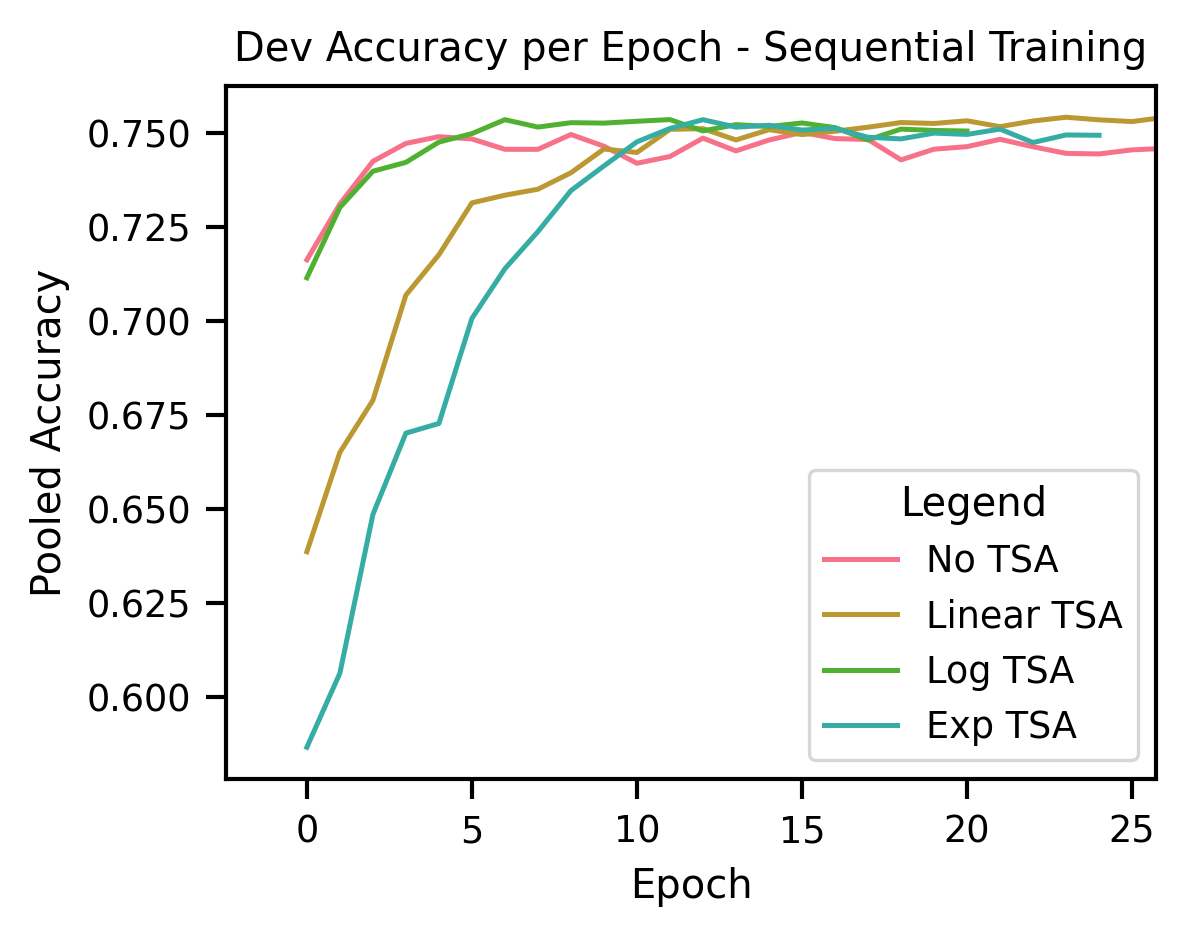
\includegraphics[height=5cm]{pics/tsa-sequential-dev.png} }}%
  \qquad
  \subfloat
  {{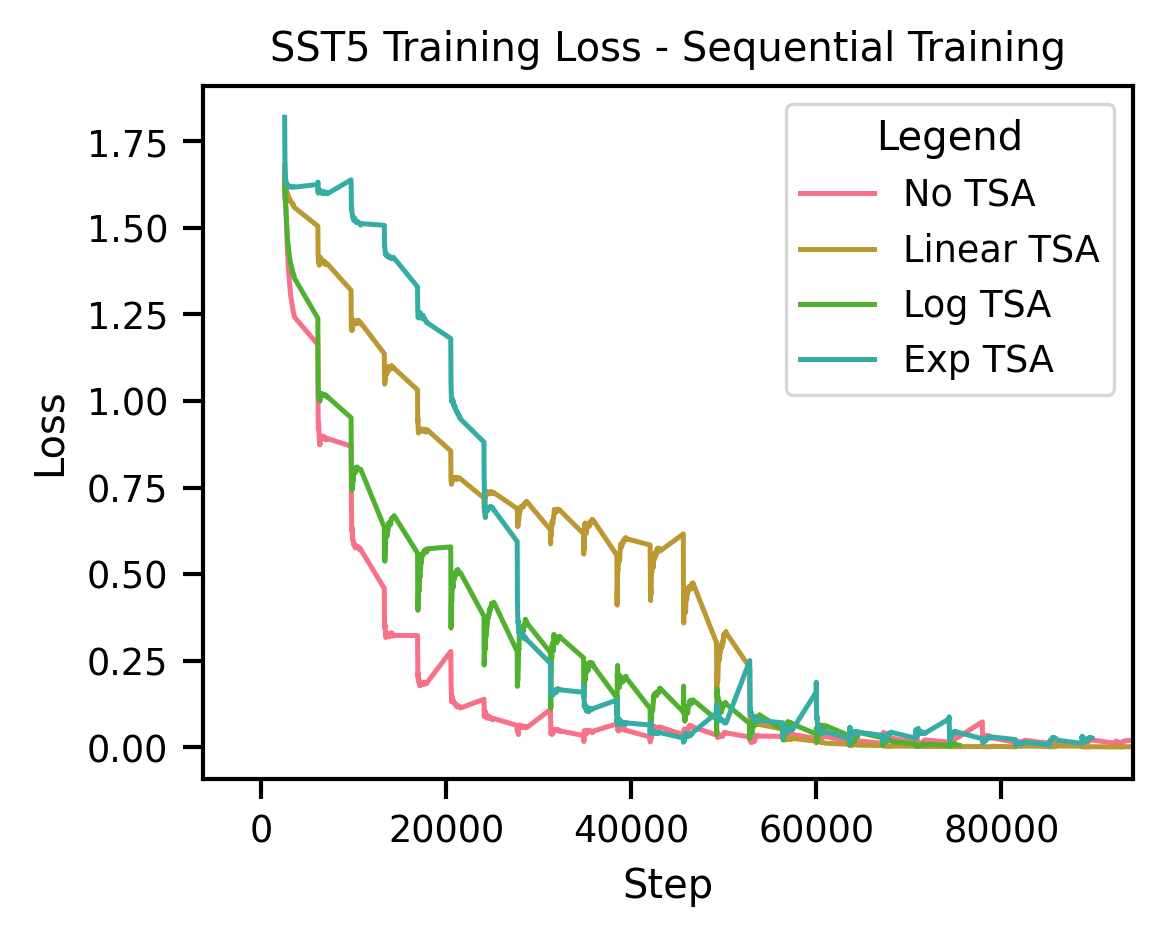
\includegraphics[height=5cm]{pics/tsa-seq-sst-loss.png} }}%
  \qquad
  \subfloat
  {{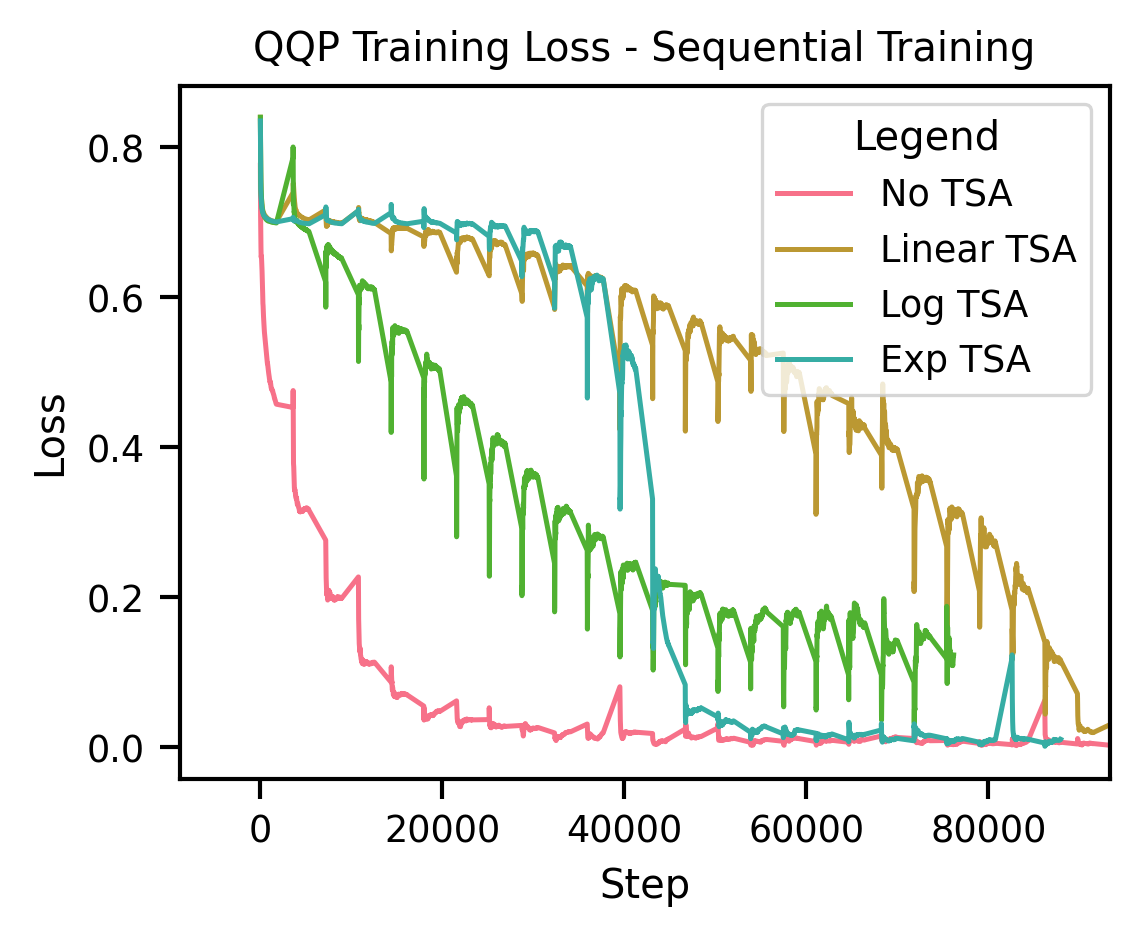
\includegraphics[height=5cm]{pics/tsa-seq-qqp-loss.png} }}%
  \qquad
  \subfloat
  {{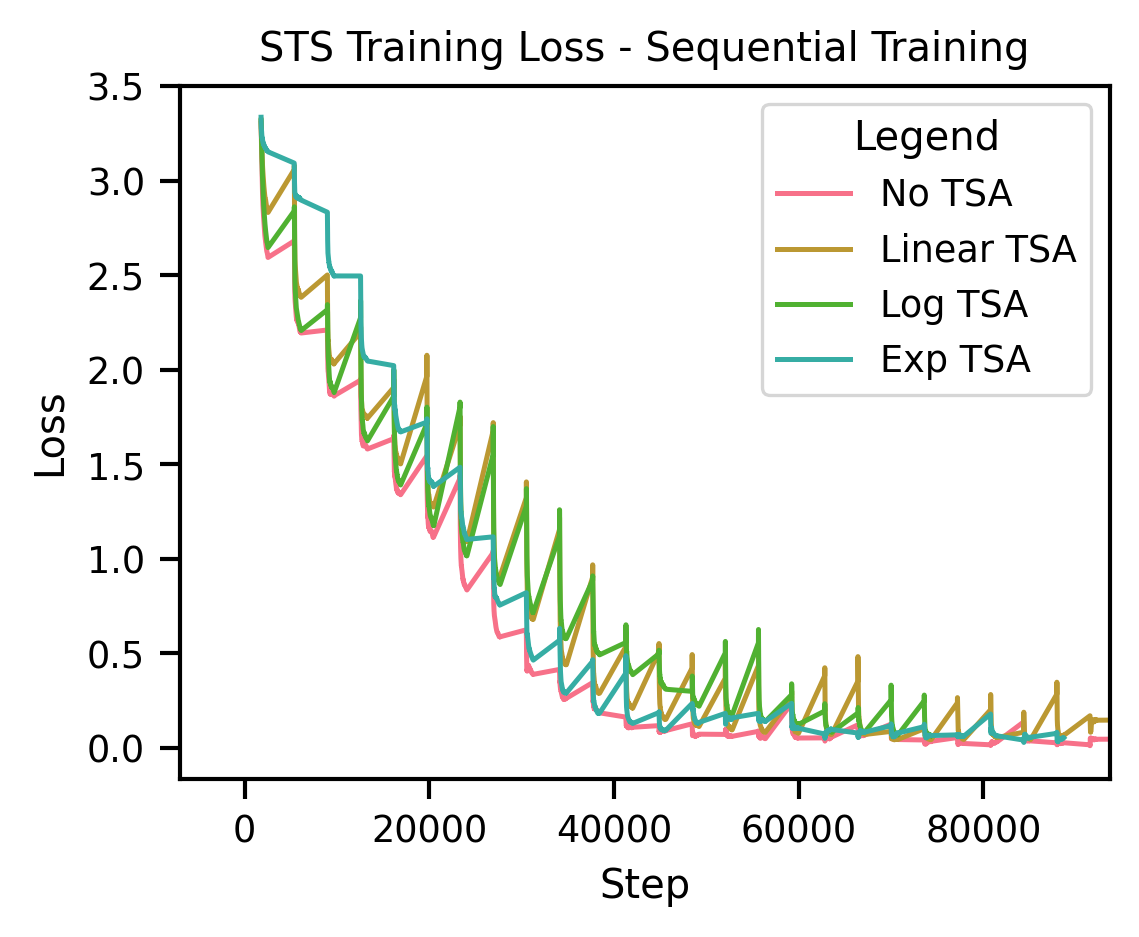
\includegraphics[height=5cm]{pics/tsa-seq-sts-loss.png} }}%
  \caption{Comparing characteristics of different TSA threshold functions - 
  Sequential Training}%
  \label{fig:tsa}%
\end{figure}

\section{Future work}
% Describe what you plan to do for the rest of the project and why.
Future steps include implementing the unsupervised loss function and experimenting with 
PLMs for data augmentation using back-translation and sentence completion. This will 
complete the UDA setup. We will also study the ratio of supervised to unsupervised samples 
to understand the minimum labeled dataset size for decent performance. Given time, we will 
explore complex task head models and hyperparameter tuning to enhance results.


\bibliographystyle{unsrt}
\bibliography{references}

\newpage
\appendix
\renewcommand{\thefigure}{A\arabic{figure}}
\renewcommand{\thetable}{A\arabic{table}}
\setcounter{figure}{0}
\setcounter{table}{0}

\section{Approaches Appendix}
% Include any additional information or analysis that is relevant to your project but not necessary in the main body of the report.
% This could include additional experiments, visualizations, or detailed derivations.
% Make sure to refer to the appendix in the main body of the report when necessary.

\subsection{Baseline extensions}
\label{sec:baseline-extensions}
\paragraph{Combining Sentence Embeddings}

We investigated two categories of architectures for combining sentence embeddings, as shown 
in Figure \ref{fig:example}. The first architecture, Pooling Separate Embeddings, derives 
a joint embedding from two separately BERT-encoded sentences. We experimented with various 
methods including simple concatenation, absolute difference (inspired by the SBERT framework 
\cite{reimers2019sentencebert}), cosine similarity, and dot product attention. 
The second architecture, 
Fused Sentence Embedding, leverages BERT's inherent training with sentence pairs separated 
by the \texttt{[SEP]} token to encode sentence context similarities. This approach fuses 
the two sentences into a single input sequence to generate a single embedding.

\begin{figure}[h]%
  \centering
  \subfloat[\centering Archetecture 1: Pooling seperate embeddings]
  {{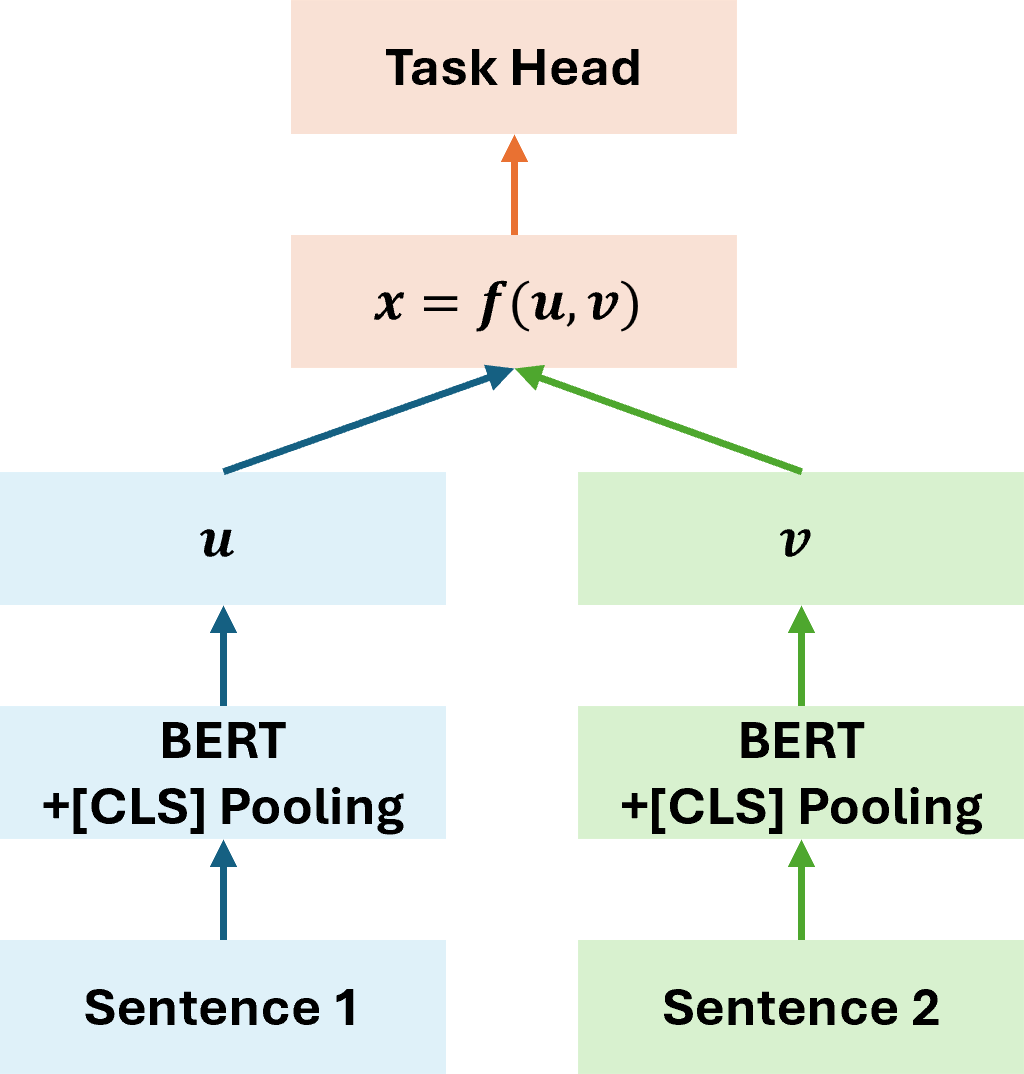
\includegraphics[height=4cm]{pics/combine_1.png} }}%
  \qquad
  \subfloat[\centering Archetecture 2: Fused sentence embedding]
  {{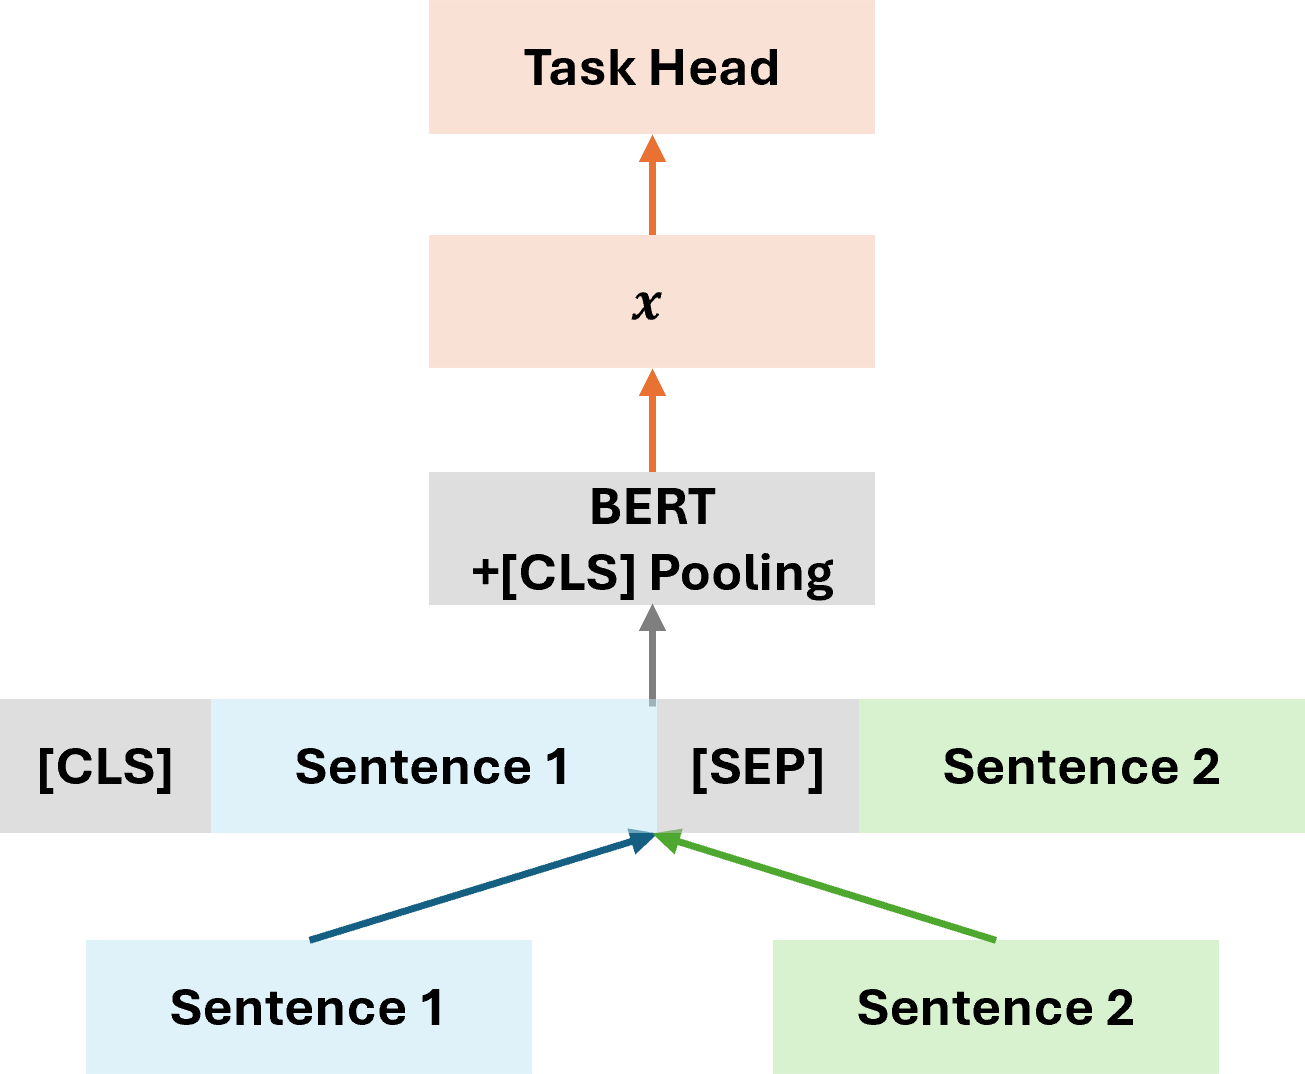
\includegraphics[height=4cm]{pics/combine_2.png} }}%
  \caption{Two architectures for sentence-pair inputs: 
  (a) Each sentence is BERT-encoded separately, then pooled into a single embedding.
  (b) Sentence-pairs are concatenated with a \texttt{[SEP]} token and BERT-encoded into 
  one embedding.
  }%
  \label{fig:example}%
\end{figure}

\paragraph{Training Strategies}
Our model optimization involved two training strategies for multiple tasks. In Sequential 
Training, each task (QQP, STS, SST) was trained sequentially within each epoch, updating 
the BERT and model parameters after each task head training. Simultaneous Training, on the 
other hand, computed and aggregated the losses for all tasks at once, updating the model 
parameters once per batch.

\subsection{Default Loss Function for UDA}
\label{sec:def-uda-loss}
Formally, given labeled dataset $L$ and unlabeled dataset $U$, we aim to learn a 
classification model $p_{\theta}$ with parameters $\theta$. This model maps input $x$ to a 
class distribution $\hat y = p_{\theta}(x)$. We denote data augmentation as $q(\cdot)$, 
where $\hat x = q(x)$ is the augmented input. Our goal is to find $\theta$ minimizing the 
loss function $J(\theta) = \mathcal{L}_{\text{sup}} + \lambda \mathcal{L}_{\text{unsup}}$, 
where $\mathcal{L}_{\text{sup}}$ is the supervised cross-entropy loss, $\mathcal{L}_{\text{unsup}}$ is 
the unsupervised loss between unlabeled and augmented data, and $\lambda$ is the 
regularization coefficient.
The default loss function is:
$$\mathcal{L} = 
- \sum_{i=1}^{|L|} y_i \log p_{\theta}(x_i)
- \lambda \sum_{j=1}^{|U|} p_{\tilde{\theta}}(x_j) \log 
\frac{p_{\tilde{\theta}}(x_j)}{p_{\theta}(\hat x_j)}
$$

\section{Results Appendix}
\subsection{Training strategies}
Simultaneous training yields similar pooled accuracy comparing with sequential training, 
with variations in single-task performance.


\begin{table}[H]
  \centering
  \caption{Comparisons of Baselines and Extensions on Dev Data, training three tasks simultaneously}
  \label{tab:baseline_ext}
  \begin{tabular}{@{}lcccc@{}}
    \toprule
    \textbf{Model}                & \multicolumn{1}{c}{\textbf{SST5}} & \multicolumn{1}{c}{\textbf{QQP}} & \multicolumn{1}{c}{\textbf{STS}} & \multicolumn{1}{c}{\textbf{\begin{tabular}[c]{@{}c@{}}Avg. Accuracy\end{tabular}}} \\ \midrule
    Baseline (last-layer only)    & 0.309                             & 0.667                            & 0.209                            & 0.527                                                                                 \\
    Arc1-Simple Concat            & 0.479                             & 0.738                            & 0.369                            & 0.634                                                                                 \\
    Arc1-Absolute difference      & 0.51                              & 0.733                            & 0.532                            & 0.670                                                                                 \\
    Arc1-Cosine Similarity        & 0.482                             & 0.533                            & 0.436                            & 0.578                                                                                 \\
    Arc1-Dot Product Attention    & \textbf{0.514}                    & 0.737                            & 0.486                            & 0.665                                                                                 \\
    Arc2-Fused Sentence Embedding & 0.507                             & \textbf{0.830}                   & \textbf{0.873}                   & \textbf{0.758}                                                                        \\ \bottomrule
    \end{tabular}
\end{table}

\end{document}
